\documentclass[]{emulateapj}
\PassOptionsToPackage{hyphens}{url}\usepackage{hyperref}
\usepackage{natbib}
\usepackage{amssymb}
\usepackage{color}
\usepackage{amsmath,mathtools}
\usepackage{epsfig}
\usepackage[FIGTOPCAP]{subfigure}
\usepackage{afterpage}
\usepackage{enumerate}
\usepackage{multirow}
\usepackage{verbatim}
\usepackage{relsize}
\usepackage{tikz}
\usetikzlibrary{shapes.geometric, arrows}
\usepackage{morefloats}
\usepackage{wasysym}

\newcommand{\noop}[1]{}
\newcommand{\note}[1]{{\color{red} #1}}
\newcommand{\cn}{\note{(cite)}}
\newcommand{\unit}[1]{\ensuremath{\, \mathrm{#1}}}
\newcommand{\mearth}{\unit{M_\oplus}}
\newcommand{\rearth}{\unit{R_\oplus}}
\newcommand{\msun}{\unit{M_\odot}}
\newcommand{\lsun}{\unit{L_\odot}}
\newcommand{\mstar}{\unit{M_\star}}
\newcommand{\rj}{\ensuremath{R_\mathrm{J}}}
\newcommand{\avg}[1]{\langle #1 \rangle}
\newcommand{\bavg}[1]{\bigg\langle #1 \bigg\rangle}
\newcommand{\tab}[1]{\hspace{.2\textwidth}\rlap{#1}}
\DeclareMathOperator*{\argmin}{arg\,min}

\shorttitle{Proxima Centauri b Water Loss}
\shortauthors{Rodrigo Luger}

\begin{document}

\title{Proxima Centauri b Water Loss}
\author{Rodrigo Luger}


\section{Intro}
\label{sec:intro}

We perform a suite of Markov Chain Monte Carlo (MCMC) runs to obtain constraints on the
present-day water content of Proxima Centauri b using the Python code package \texttt{emcee}
\citep{ForemanMackey13}. MCMC allows one to sample from multi-dimensional probability 
distributions that are difficult or impossible to obtain directly, which is the case for
the ensemble of parameters that control the evolution of the planet surface water content
in \texttt{VPLANET}. In this section, we develop a framework for inferring the probability 
distributions of these parameters conditioned on empirical data and our understanding
of the physical processes at play.

The input parameters to our model make up the state vector $\mathbf{x}$:
%
\begin{align}
\label{eq:mcmcx}
\mathbf{x} = \{f_\mathrm{sat}, t_\mathrm{sat}, \beta_\mathrm{xuv}, M_\star, t_\star, a, m\},
\end{align}
%
corresponding, respectively, to the stellar mass, the XUV saturation fraction, the XUV saturation timescale,
the XUV power law exponent, the stellar age, the semi-major axis of the planet, and the
mass of the planet. Given a value of $\mathbf{x}$, \texttt{VPLANET} computes the evolution of the system from
time $t = 0$ to $t = t_\star$, yielding the output vector $\mathbf{y}$:
%
\begin{align}
\label{eq:mcmcy}
\mathbf{y}(\mathbf{x}) = \{L_\star, L_\mathrm{xuv}, t_\mathrm{RG}, m_\mathrm{H}, m_\mathrm{H_2O}, P_\mathrm{O_2}\},
\end{align}
%
corresponding, respectively, to the stellar luminosity, the stellar XUV luminosity, the duration of the 
runaway greenhouse phase, the mass of the
planet's hydrogen envelope, the mass of water remaining on its surface, and the amount of oxygen (expressed
as a partial pressure) retained
in either the atmosphere or the surface/mantle, all of which are evaluated at $t = t_\star$ (i.e., the present day). 
Additional parameters that control the evolution of the 
planet (initial water content, XUV absorption efficiency, etc.) are held fixed in individual runs; see below.

Our goal in this section is to derive posterior distributions for $\mathbf{y}$ (and in particular for $m_\mathrm{H_2O}$) 
given prior information on both 
$\mathbf{x}$ and $\mathbf{y}$. Some parameters---such as the present-day stellar luminosity---are well-constrained,
while others are less well-known and will thus be informed primarily by our choice of prior. This is the case for
the XUV saturation fraction, saturation timescale, and power law exponent, which have been studied in detail 
for solar-like stars \citep{Ribas05} but are poorly constrained for M dwarfs. \note{More info on them here...}
We therefore use flat-log priors for the saturation fraction and timescale, enforcing
$-5 \leq \log(f_\mathrm{sat}) \leq -2$ and $-0.3 \leq \log(t_\mathrm{sat} / \mathrm{Gyr}) \leq 1$. We use
a Gaussian prior for the XUV power law exponent, with a mean of 1.23, the value derived by \citep{Ribas05} for
solar-like stars: $\beta_\mathrm{xuv} \sim \mathcal{N}(-1.23, 0.1)$. We choose an ad hoc standard deviation
$\sigma = 0.1$ and verify \emph{a posteriori} that our results are not sensitive to this choice. As we show
below, $\beta_\mathrm{xuv}$ does not strongly correlate with the total water lost or total
amount of oxygen that builds up on the planet.

We also use a flat prior for the stellar mass ($0.1 \leq M_\star / \mathrm{M}_\oplus \leq 0.15$).
Although stronger constraints on the stellar mass exist \cn, these are derived indirectly from mass-luminosity relations; we thus
enforce a prior on the present-day luminosity to constrain the value of $M_\star$ via our stellar evolution model (see below).
We enforce a Gaussian prior on the stellar age $t_\star \sim \mathcal{N}(4.8, 1.4^2)$ Gyr based on the constraints discussed
in \S\cn. 

Our prior on the semi-major axis $a$ is a combination of a Gaussian prior on the orbital period, 
$P \sim \mathcal{N}(11.186, 0.002^2)$ days \citep{AngladaEscude16}, and the stellar mass prior. 
Finally, our prior on the planet mass $m$ combines the empirical minimum mass distribution,
$m\sin i \sim \mathcal{N}(1.27, 0.18^2)$ M$_\oplus$ \citep{AngladaEscude16}, and the a priori inclination distribution
for randomly aligned orbits, 
$\sin i \sim \mathcal{U}(0, 1)$, where $\mathcal{U}$ is a uniform distribution \citep[e.g.,][]{Luger17}.

We further condition our model on measured values of the stellar luminosity $L_\star$ and 
stellar XUV luminosity $L_\mathrm{xuv}$. We take
$L_\star \sim \mathcal{N}(1.65, 0.15) \times 10^{-3}$ L$_\odot$ \citep{Demory09} and 
$\log L_\mathrm{xuv} \sim \mathcal{N}(-6.36, 0.3^2)$. We base the latter on \cite{Ribas16}, who compiled a comprehensive
list of measurements of the emission of Proxima Centauri in the wavelength range 0.6--118 nm. Summing the fluxes over
this range and neglecting the contribution of flares, we obtain an XUV flux at Proxima Centauri b 
$F_\mathrm{xuv} \approx 252\ \mathrm{erg\ cm^{-2}\ s^{-1}}$, corresponding to $\log L_\mathrm{xuv} = -6.36$ for $a = 0.0485$ AU. Given the
lack of uncertainties for many of the values compiled in \cite{Ribas16} and the fact that some of those estimates
are model extrapolations, it is difficult to establish a reliable error estimate for this value. We make the 
ad hoc but conservative choice $\sigma = 0.3$ dex, noting that the three measurements that inform the X-ray luminosity 
of the star in \cite{Ribas16} (which dominates its XUV emission) have a spread corresponding to $\sigma = 0.2$ dex. 
However, more rigorous constraints on the XUV emission of Proxima Cen with reliable uncertainties are direly needed
to obtain more reliable estimates of water loss from Proxima Cen b.

Given these constraints, we wish to find the posterior distribution of each of the parameters in Equations~(\ref{eq:mcmcx}) 
and~(\ref{eq:mcmcy}). We thus define our likelihood function $\mathcal{L}$ for a given state vector $\mathbf{x}$ as
%
\begin{align}
\ln \mathcal{L}(\mathbf{x}) = &- \frac{1}{2}\left[\frac{(L_\mathrm{\star}(\mathbf{x}) - L_\mathrm{\star})^2}{\sigma_{L_\star}^2}
                               - \frac{(L_\mathrm{xuv}(\mathbf{x}) - L_\mathrm{xuv})^2}{\sigma_{L_\mathrm{xuv}}^2}\right]
                                 \nonumber\\
                              &+ \ln \mathrm{Prior}(\mathbf{x}) + C,
\end{align}
%
where $L_\mathrm{\star}(\mathbf{x})$ and $L_\mathrm{xuv}(\mathbf{x})$ are, respectively, the model predictions for the present-day 
stellar luminosity and stellar XUV luminosity given the state vector $\mathbf{x}$, $L_\mathrm{\star}$ and $L_\mathrm{xuv}$ are
their respective observed values, and $\sigma_{L_\star}^2$ and $\sigma_{L_\mathrm{xuv}}^2$ are the uncertainties on those observations. The
$\ln \mathrm{Prior}(\mathbf{x})$ term is the prior probability and $C$ is an arbitrary normalization constant. Expressed in this form,
the observed values of $L_\mathrm{\star}$ and $L_\mathrm{xuv}$ are our ``data,'' while the constraints on the other parameters
are ``priors,'' though the distinction is purely semantic.

\begin{figure}[hbt]
  \begin{center}
      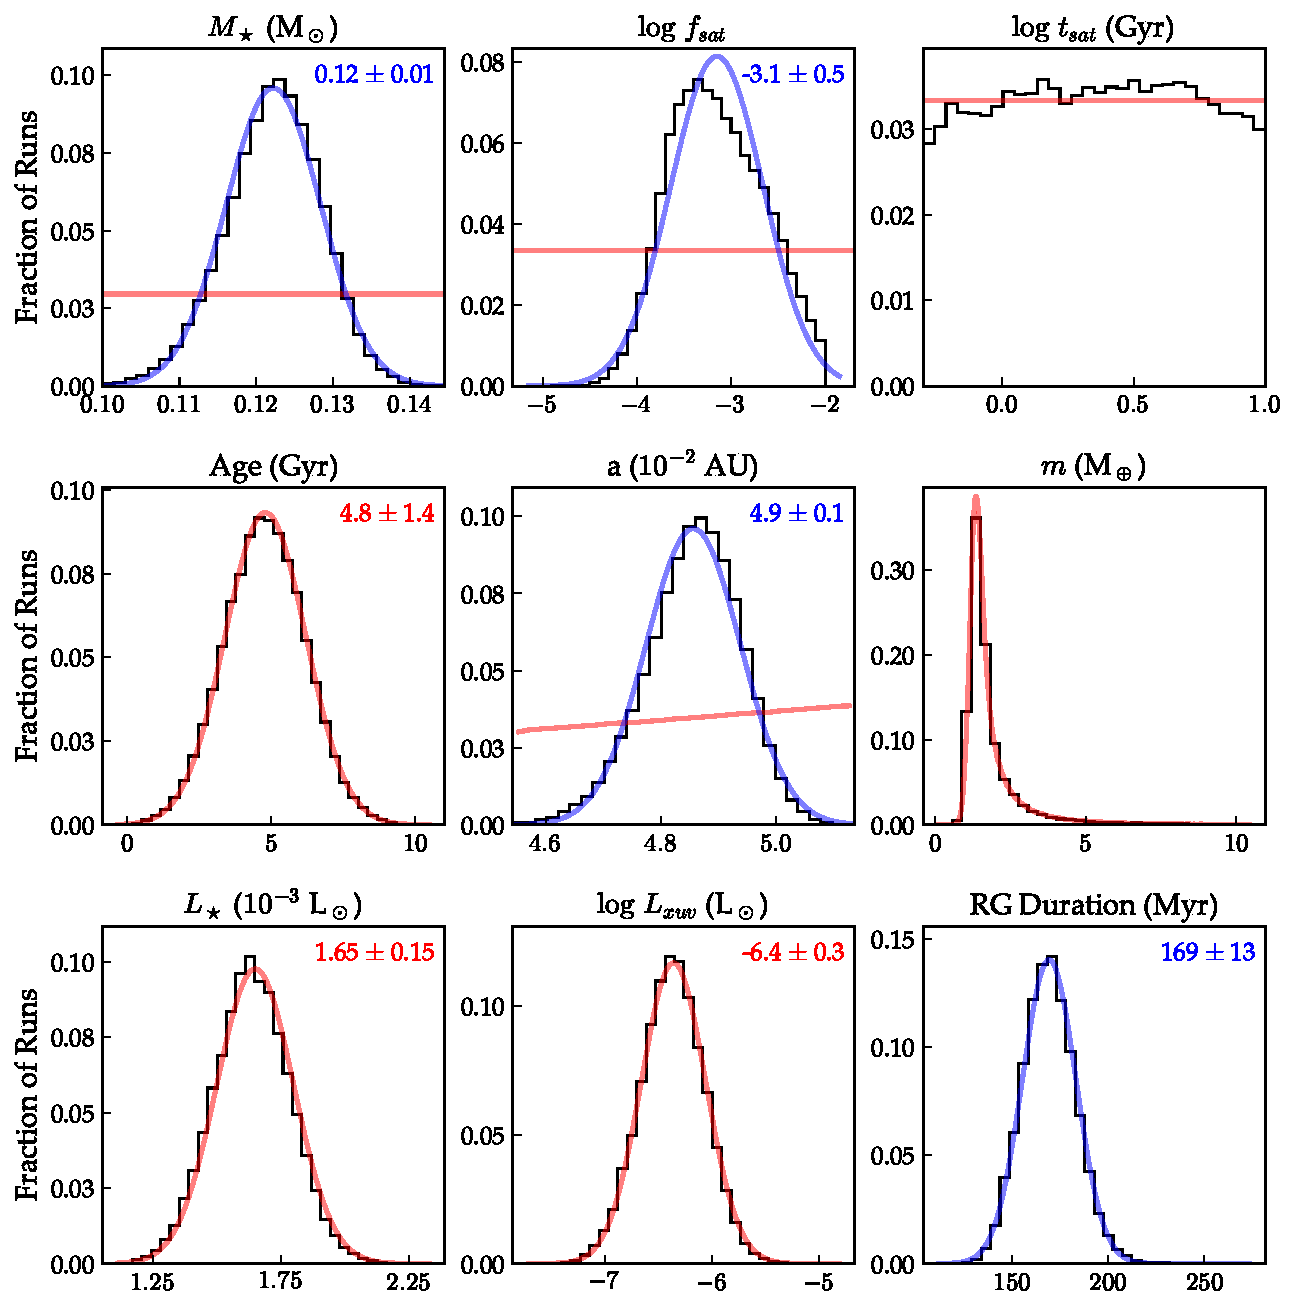
\includegraphics[width=0.45\textwidth]{figures/star_posteriors.pdf}
       \caption{Posterior distributions for the various stellar parameters used in the model. The first eight
                parameters are model inputs, with their corresponding priors shown in red. The combination of
                these priors and the physical models in \texttt{VPLANET} constrain the stellar and planetary
                parameters shown in this section. Blue curves show Gaussian fits to the posterior distributions,
                with the mean and standard deviation indicated at the top right.
                The last panel shows the duration of the runaway greenhouse
                phase for Proxima Centauri b, one of the model outputs, which we find to be 169 $\pm$ 13 Myr.}
     \label{fig:star_posteriors}
  \end{center}
\end{figure}

Given this likelihood function, we use MCMC to obtain the posterior probability distributions for each of the parameters
of interest. We draw each of the $\mathbf{x}$ from their respective prior distributions and run 40 parallel chains of 5,000 
steps each, discarding the first 500 steps as burn-in. The marginalized posterior distributions for the stellar mass, saturation fraction,
saturation timescale, age, semi-major axis, planet mass, present-day stellar luminosity, present-day stellar XUV luminosity, and 
duration of the runaway greenhouse are shown in Figure~\ref{fig:star_posteriors} as the black histograms. The red curves 
indicate our priors/data, and the purple curve is a Gaussian fit to the runaway greenhouse duration posterior,
yielding $t_\mathrm{RG} = 169 \pm 13$ Myr.

By construction, the planet mass, stellar age, present-day stellar luminosity, and present-day stellar XUV luminosity posteriors reflect
their prior distributions. As mentioned above, the stellar mass posterior is entirely informed by the luminosity posterior via the
\cite{YonseiYale13} stellar evolution tracks. The stellar mass in turn constrains the semi-major axis (via the prior on the period and
Kepler's laws). The XUV saturation fraction is fairly well constrained by the present-day XUV luminosity; a log-normal fit
to its posterior yields $\log\ f_\mathrm{sat} = -3.1 \pm 0.5$, which is fully consistent with the observation that M dwarfs
saturate at or below $\log\ f_\mathrm{sat} \approx -3$ \cn. The longer tail at high $f_\mathrm{sat}$ results from the fact that
this parameter is strongly correlated with the saturation timescale, $t_\mathrm{sat}$ (see Figure~\ref{fig:corner} below). If
saturation is short-lived, the initial saturation fraction must be higher to match the present-day XUV luminosity. Interestingly,
our runs do not provide any constraints on $t_\mathrm{sat}$, whose value is equally likely (in log space) across the range 
$[0.5, 10]$ Gyr. Finally, the posterior for the XUV power law exponent $\beta_\mathrm{xuv}$ (not shown in the Figure) is 
the same as the adopted prior, as the present data is insufficient to constrain it.

\begin{figure}[hbt]
  \begin{center}
      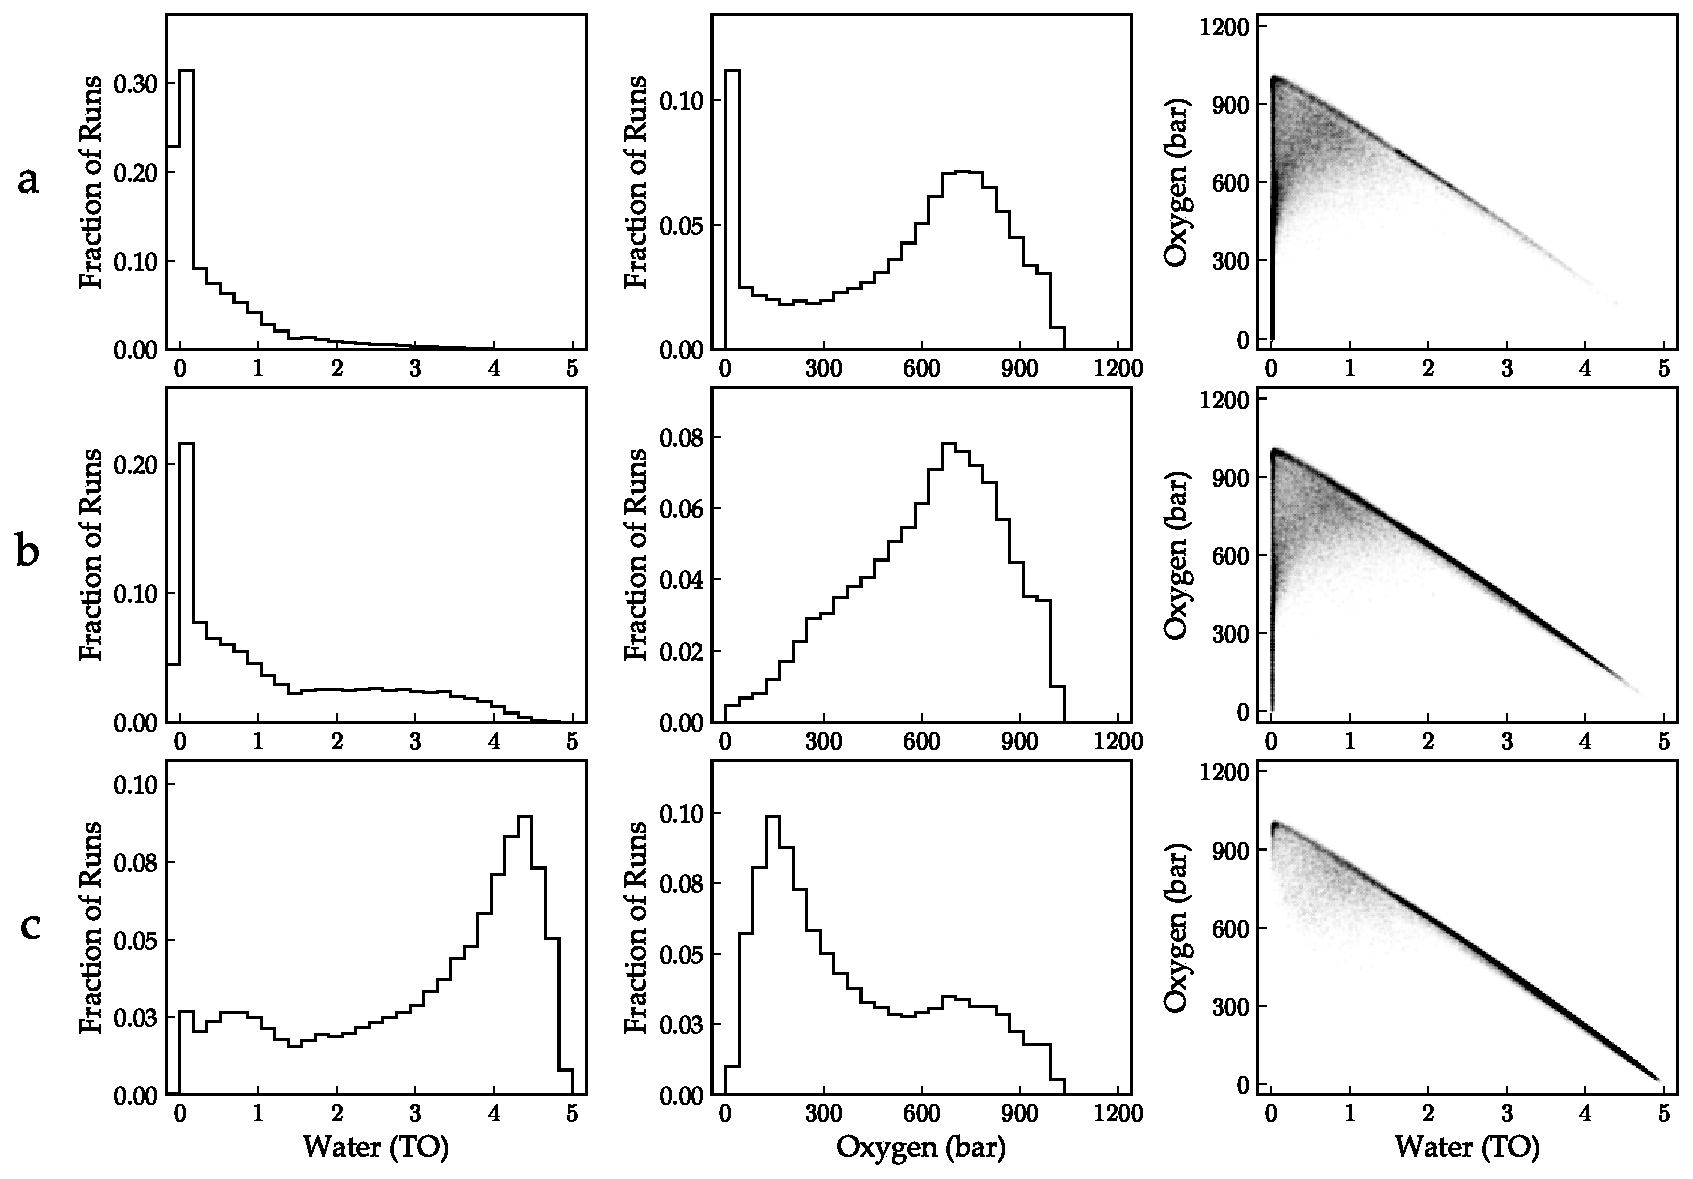
\includegraphics[width=0.45\textwidth]{figures/planet_epsilon.pdf}
       \caption{Marginalized posteriors for the present-day water content (left) and atmospheric oxygen
       pressure (center) on Proxima Cen b. The joint posteriors for these two parameters are shown at the 
       right. \textbf{(a)} Posteriors for the default run ($m_\mathrm{H_2O}^0 = 5$ TO, $m_\mathrm{H}^0 = 0$,
       $\epsilon_\mathrm{xuv} = 0.15$, $\zeta_\mathrm{O_2} = 0$). \textbf{(b)} Same as (a), but for
       $\epsilon_\mathrm{xuv} = 0.05$. \textbf{(c)} Same as (a), but for
       $\epsilon_\mathrm{xuv} = 0.01$. For $\epsilon_\mathrm{xuv} \gtrsim 0.05$, the planet loses close to
       5 TO of water and builds up between 500 and 900 bars of O$_2$ in most runs. For $\epsilon_\mathrm{xuv} \sim 0.01$,
       the planet loses less water and builds up less O$_2$, though the loss of more than 1 TO is still likely.
       }
     \label{fig:planet_epsilon}
  \end{center}
\end{figure}

The two quantities that are of the most interest to us --- the final water content $m_\mathrm{H_2O}$ and final O$_2$ atmospheric 
pressure $P_\mathrm{O_2}$ of Proxima Cen b --- depend on four additional parameters we must specify: the initial water content $m_\mathrm{H_2O}^0$, the initial hydrogen 
mass $m_\mathrm{H}^0$ (if the planet formed with a primordial envelope), the XUV escape efficiency $\epsilon_\mathrm{xuv}$, and
the O$_2$ uptake efficiency $\zeta_\mathrm{O_2}$ of the planet surface. In principle, planet formation models could provide
priors on $m_\mathrm{H_2O}^0$ and $m_\mathrm{H}^0$, but such models depend on additional parameters that are unknown or poorly 
constrained. The same is true for the XUV escape efficiency, which can be modeled as in \cite{Ribas16}, and the rate of
absorption of O$_2$ at the surface, which can be computed as in \cite{Schaefer2016}. However, given the large number of unknown
parameters needed to constrain these four parameters, for simplicity we perform independent MCMC runs for fixed combinations
of these. By doing this, we circumvent potential biases arising from incorrect priors on these parameters while still
highlighting how our results scale for different assumptions about their values.

In the runs discussed below, our default values are $m_\mathrm{H_2O}^0 = 5$ TO, $m_\mathrm{H}^0 = 0\ \mathrm{M_\oplus}$,
$\epsilon_\mathrm{xuv} = 0.15$, and $\zeta_\mathrm{O_2} = 0$, and we vary each of these parameters in turn. 
Figure~\ref{fig:planet_epsilon} shows the marginalized posterior distributions for the present-day water content (left column)
and present-day O$_2$ atmospheric pressure (middle column), as well as a joint posterior for the two parameters (right column)
for three different values of $\epsilon_\mathrm{xuv}$: \textbf{(a)} 0.15, \textbf{(b)} 0.05, and \textbf{(c)} 0.01. In the first
two cases, the planet loses all or nearly all of the 5 TO it formed with, building up several hundred bars of O$_2$ (with
distributions peaking at about 700 bars and with a spread of several hundred bars). For $\epsilon_\mathrm{xuv} = 0.15$, about
10\% of runs result in no substantial oxygen remaining in the atmosphere; in these runs, the escape was so efficient as to
remove all of the O$_2$ along with the escaping $H$. In the final case, the amount of water lost is significantly smaller:
about 2 TO on average, with a peak in the distribution corresponding to a loss of about 0.8 TO. The amount of O$_2$
remaining is similarly smaller, but still exceeding 100 bars and with similar spread as before. Finally, the joint posterior
plots emphasize how correlated the present-day water and oxygen content of Proxima Cen b are. Since the rate at which
oxygen builds up in the atmosphere is initially constant at first \citep{LugerBarnes15}, and since the amount of water
lost scales with the duration of the escape period, there is a tight linear correlation between the two quantities
(lower right hand corner of the joint posterior plots). However, as the atmospheric mixing ratio of oxygen increases,
the rate at which hydrogen escapes---and thus the rate at which oxygen is produced---begins to decrease, leading to a break
in the linear relationship once $\sim$ 600--700 bars of oxygen build up and leading to the peak in the O$_2$ posteriors
at around that value.

\begin{figure}[hbt]
  \begin{center}
      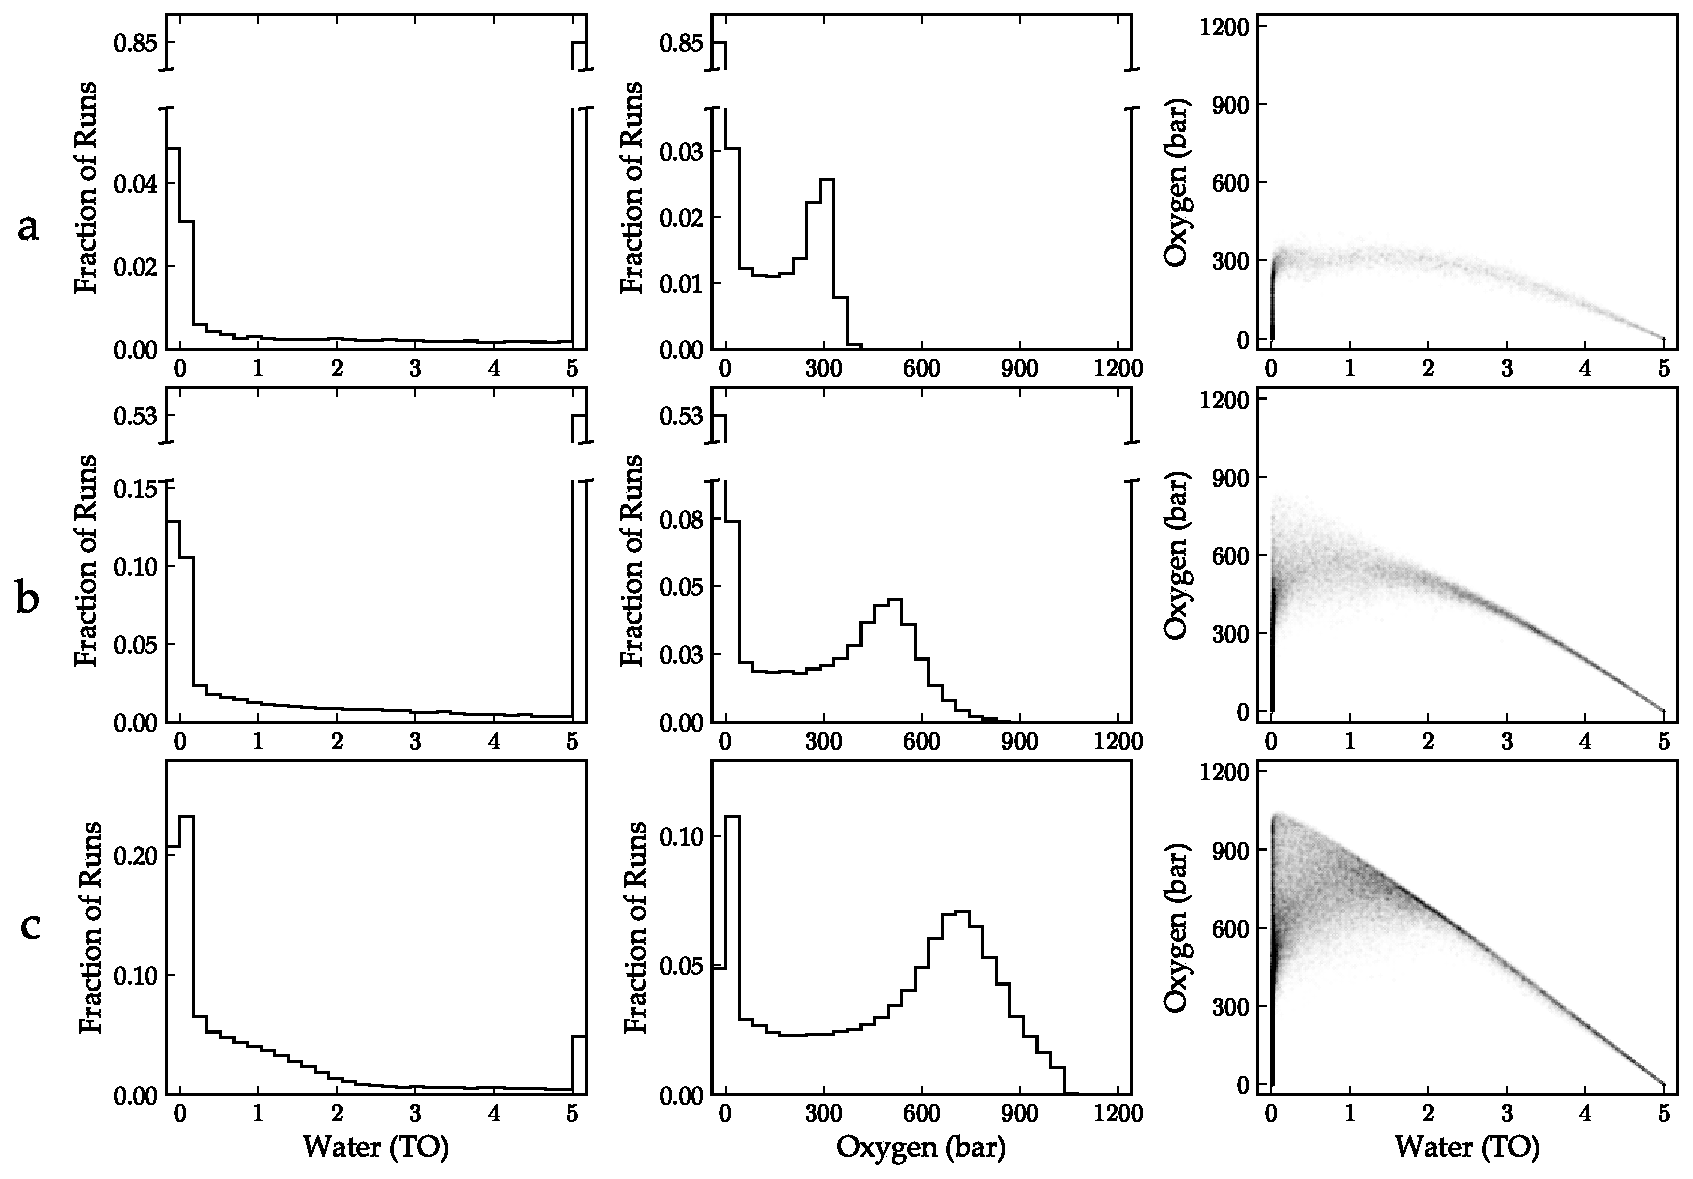
\includegraphics[width=0.45\textwidth]{figures/planet_hydrogen.pdf}
       \caption{Similar to Figure~\ref{fig:planet_epsilon}, but this time varying the initial mass of the primordial
       hydrogen envelope of Proxima Cen b. Other parameters are set to their default values. The initial mass of hydrogen
       is $m_\mathrm{H}^0 =$ \textbf{(a)} $0.01\ \mathrm{M_\oplus}$, \textbf{(a)} $0.001\ \mathrm{M_\oplus}$, and
       \textbf{(a)} $0.0001\ \mathrm{M_\oplus}$. Note the broken axes in the first two rows. In the first two cases,
       no water is lost in more than half of the runs; in such cases, a thin hydrogen envelope remains today. In the
       final case, most planets lost all their hydrogen and all their water. In order to prevent the runaway loss
       of its water, Proxima Cen b must have formed with more than 0.01\% of its mass in the form of a hydrogen envelope.
       }
     \label{fig:planet_hydrogen}
  \end{center}
\end{figure}

In Figure~\ref{fig:planet_hydrogen} we explore the effect of varying the initial hydrogen content of the planet.
From top to bottom, the rows correspond to initial hydrogen masses equal to 0.01, 0.001, and 0.0001~$\mathrm{M_\oplus}$.
In the first two cases, the effect of the envelope is clear, as most planets lose no water and build up no oxygen.
These are mostly cases in which a portion of the hydrogen envelope remains at the present day. However, if the
initial hydrogen mass is on the order of 0.0001~$\mathrm{M_\oplus}$ (corresponding to roughly 100 times Earth's
total atmospheric mass), the shielding effect of the envelope is 
almost negligible; compare panel \textbf{(c)} to the top panel in Figure~\ref{fig:planet_epsilon} (the default run).
In this case, most of the water is lost to space in the majority of the runs.

\begin{figure}[hbt]
  \begin{center}
      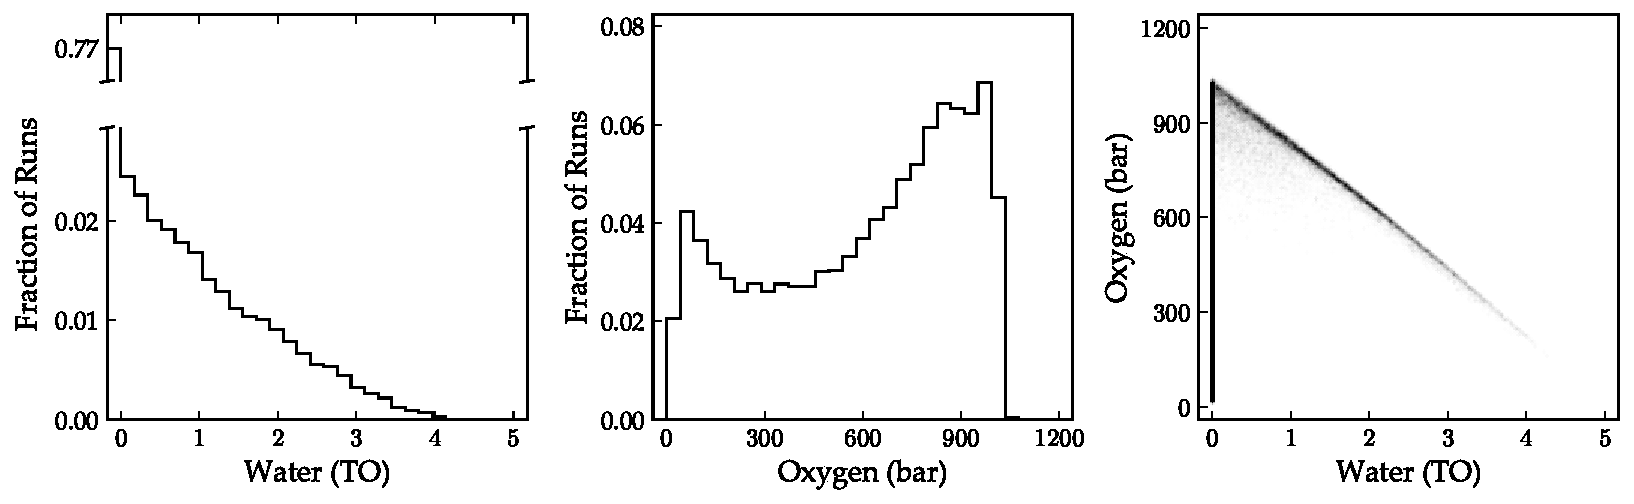
\includegraphics[width=0.45\textwidth]{figures/planet_magma.pdf}
       \caption{Planet posteriors (magma).}
     \label{fig:planet_hydrogen}
  \end{center}
\end{figure}



\begin{figure}[hbt]
  \begin{center}
      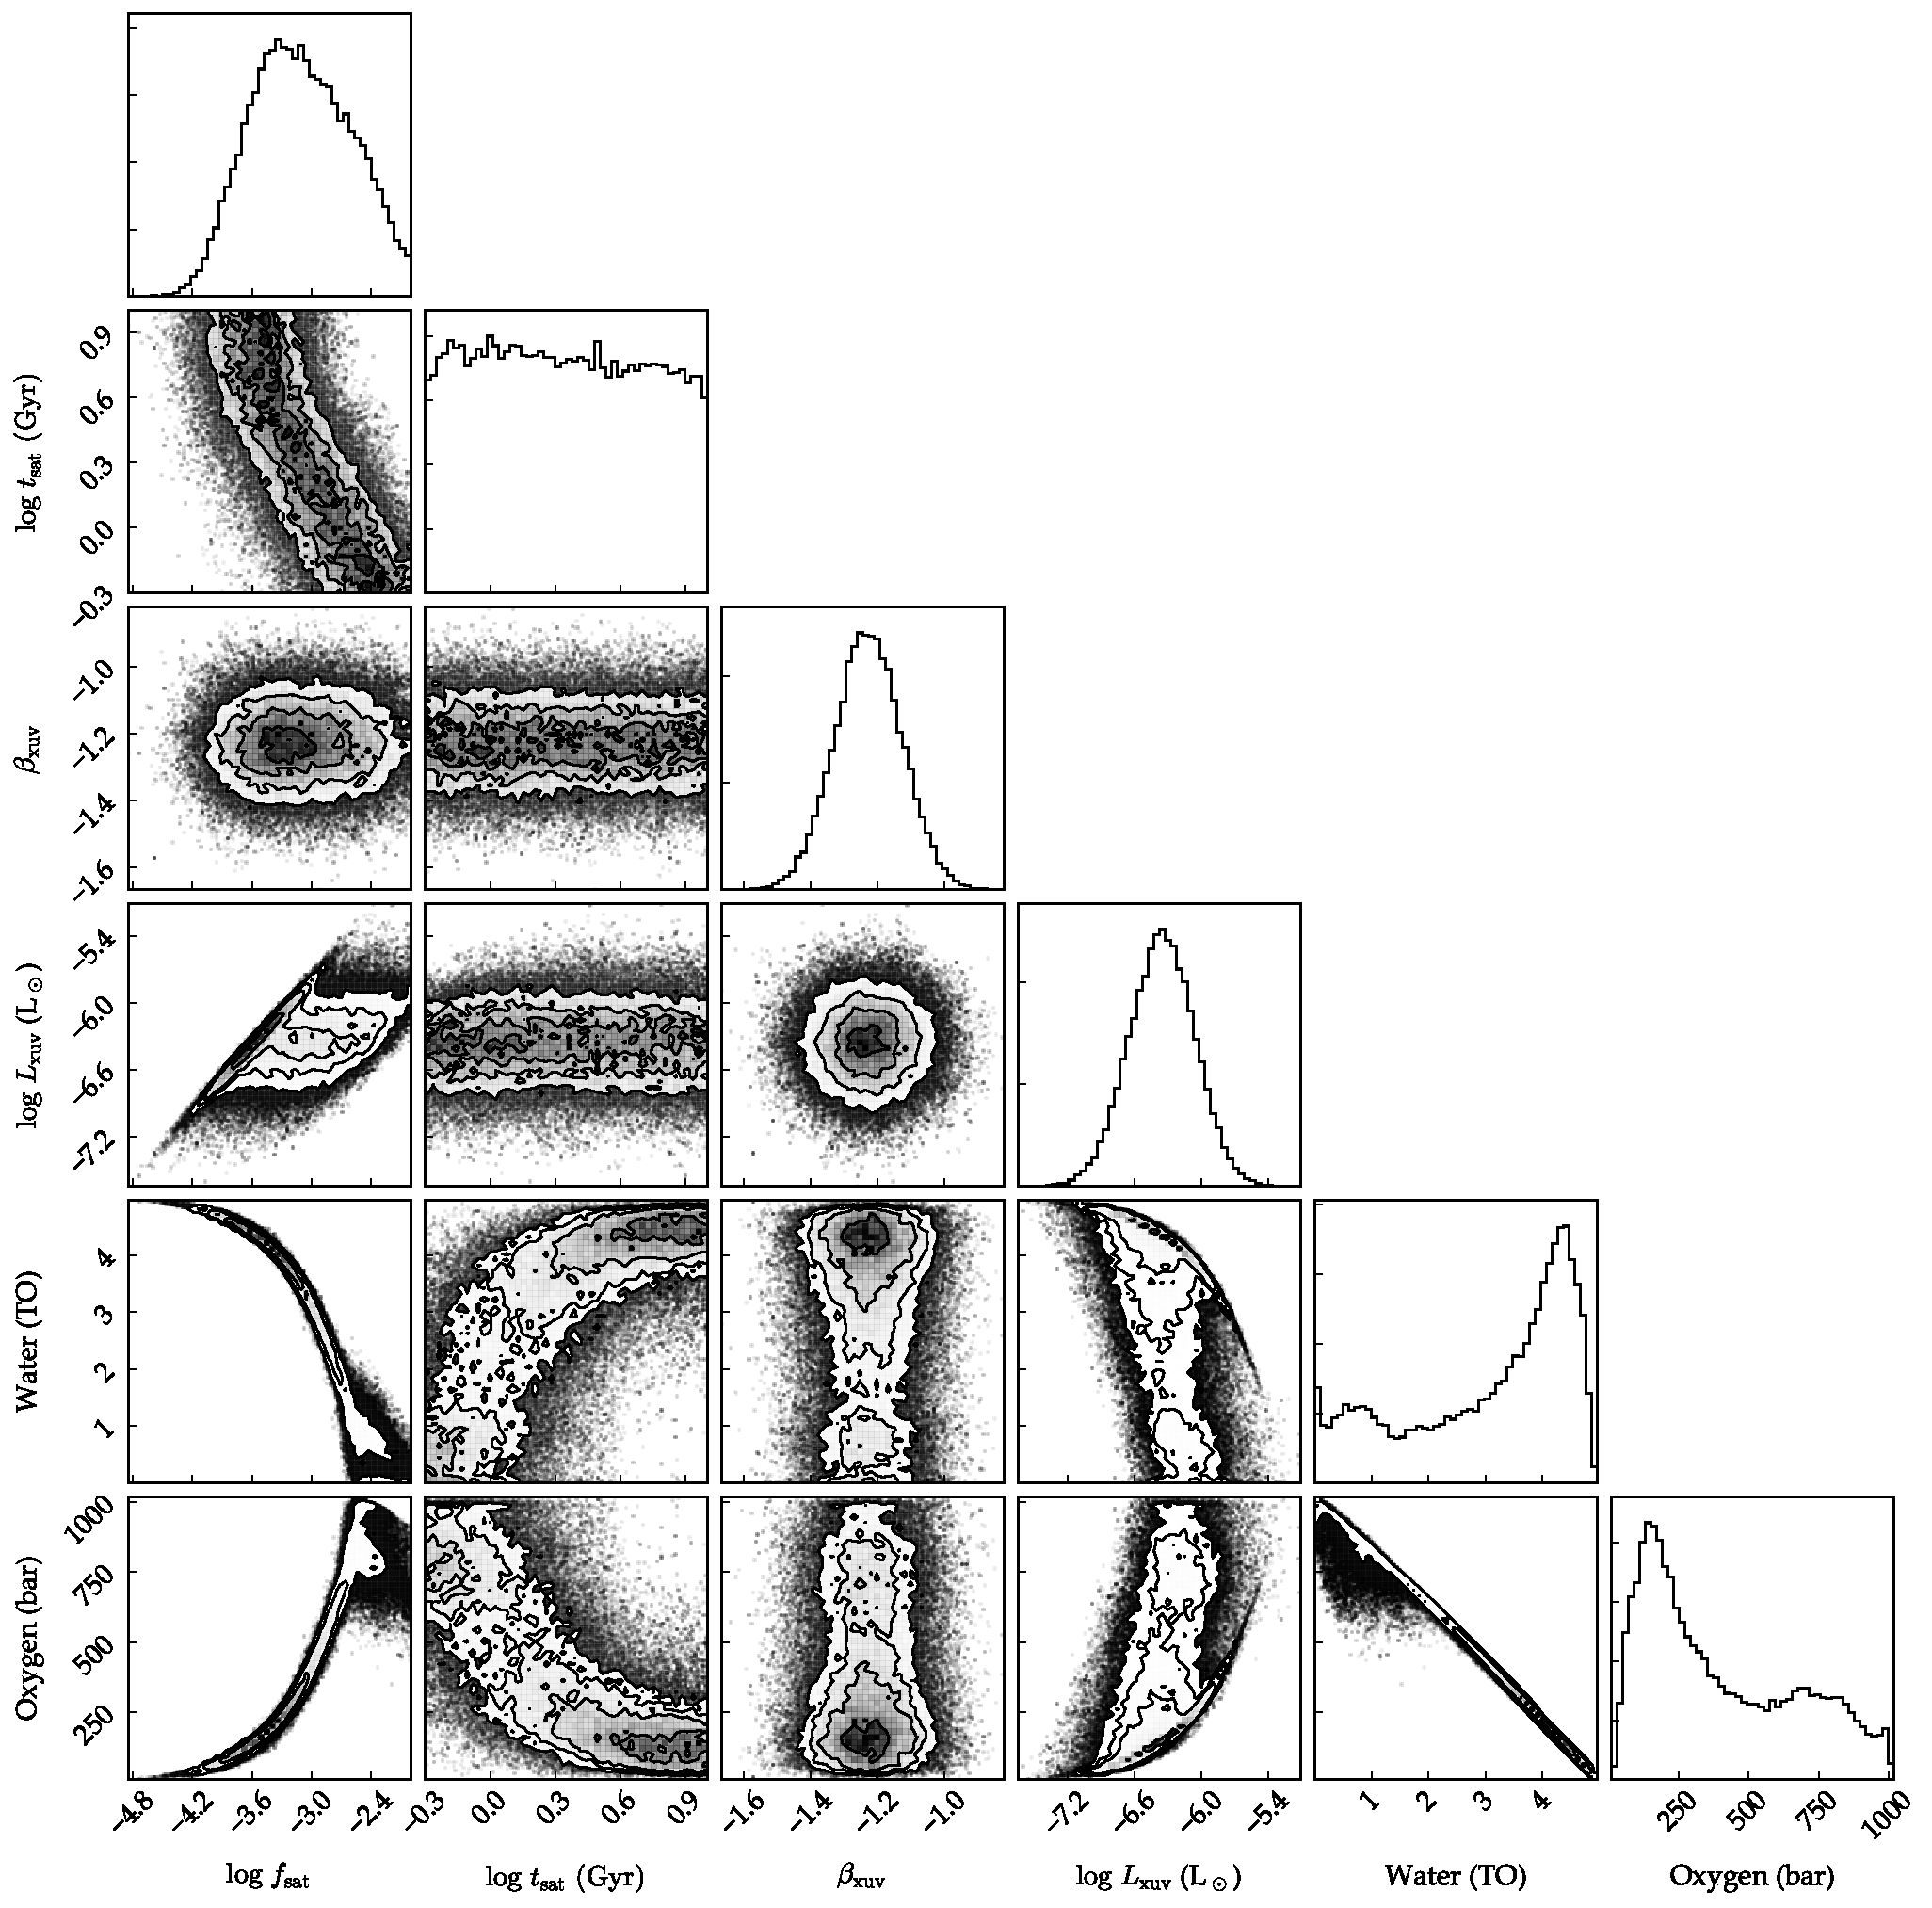
\includegraphics[width=0.45\textwidth]{figures/corner.pdf}
       \caption{Correlations. Beta isn't correlated with water because it's too late to matter.}
     \label{fig:corner}
  \end{center}
\end{figure}

\clearpage
\bibliographystyle{apj}
\bibliography{uncert}

\end{document}